%\begin{frame}
%    \frametitle{One-shot optimisation}
%
%    So far we have always first reduced the problem, i.e. eliminated the PDE-constraint, and then solved the reduced system.
%    At each optimisation iteration, we solve the forward PDE at least once. For highly non-linear PDEs, it seems unnecessary to
%    perform this solve, in particular when still far away from the optimal solution.
%
%    An alternative way is to solve the original problem directly, known as one-shot optimisation.
%
%\end{frame}
\begin{frame}
    \frametitle{One-shot optimisation}
    \begin{figure}
    \begin{center}
        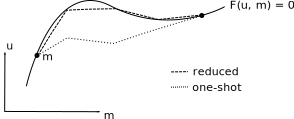
\includegraphics[width=1.0\textwidth]{pdf/one-shot} 
    \end{center}
    \end{figure}

\end{frame}



\begin{frame}
    \frametitle{One-shot optimisation}

    Consider
    \begin{equation*}
    \min_{u, m} J(u, m)
    \end{equation*}
    subject to:
    \begin{equation*}
    F(u, m) = 0.
    \end{equation*}

    \onslide<2->{
    \begin{block}{One-shot solution strategy}
    \begin{enumerate}
        \item Form Lagrangian $\mathcal L$
            \only<3>{\color{red}}
            \only<3->{
                $= J(u, m) + \left<\lambda, F(u, m)\right>$
                with Lagrange multipler $\lambda$.
                \color{black}
            }
        \item Set the derivative of $\mathcal L$ to $0$ (optimality conditions) 
            \only<4>{\color{red}}
            \only<4->{
                \begin{equation*}
                    \frac{\textrm{d} \mathcal L}{\textrm{d}u} = 0, \quad
                    \frac{\textrm{d} \mathcal L}{\textrm{d}m} = 0, \quad 
                    \frac{\textrm{d} \mathcal L}{\textrm{d}\lambda} = 0
                \end{equation*}
            }
            \color{black}
        \item Solve the resulting system 
            \only<5->{
                \color{red}for $u, m, \lambda$ simultaneously!
            }
        \color{black}
        \end{enumerate}
    \end{block}
}
\end{frame}

\begin{frame}[fragile]
  \frametitle{One-shot Hello World!}
  \begin{equation*}
        \min_{u, f} \frac{1}{2} \int_\Omega \| u - u_d\|^2\dx + \frac{\alpha}{2} \int_\Omega \| f \|^2\dx 
  \end{equation*}
  subject to:
  \begin{equation*}
      - \Delta u = f \,\,\, \quad \mbox{in } \Omega
    %u &= u_0 \quad \mbox{on } \partial \Omega
  \end{equation*}

  \onslide<2->{
      \begin{block}{1. Lagrangian}
  \begin{equation*}
        \mathcal L = \frac{1}{2} \int_\Omega \| u - u_d\|^2\dx + \frac{\alpha}{2} \int_\Omega \| f \|^2\dx 
        + \int_\Omega \lambda (- \Delta u - f) \dx
  \end{equation*}
  \end{block}

  }
\end{frame}

\begin{frame}[fragile]
  \frametitle{One-shot Hello World!}
  \begin{equation*}
        \min_{u, f} \frac{1}{2} \int_\Omega \| u - u_d\|^2\dx + \frac{\alpha}{2} \int_\Omega \| f \|^2\dx 
  \end{equation*}
  subject to:
  \begin{equation*}
      - \Delta u = f \,\,\, \quad \mbox{in } \Omega
    %u &= u_0 \quad \mbox{on } \partial \Omega
  \end{equation*}

      \begin{block}{1. Lagrangian}
  \begin{equation*}
        \mathcal L = \frac{1}{2} \int_\Omega \| u - u_d\|^2\dx + \frac{\alpha}{2} \int_\Omega \| f \|^2\dx 
        + \int_\Omega \lambda (- \Delta u - f) \dx
  \end{equation*}
  \end{block}

  \begin{block}{Code}
\begin{python}
L = 0.5*inner(u-ud, u-ud)*dx
  + 0.5*alpha*inner(f, f)*dx 
  + inner(grad(u), grad(lmbd))*dx
  - f*lmbd*dx
\end{python}
\end{block}
\end{frame}

\begin{frame}[fragile]
  \frametitle{2. Optimality (KKT) conditions}
     
      \only<1>{
  \begin{equation*}
    \begin{aligned}
        \frac{\partial \mathcal L}{\partial u}\tilde u &= 0 && \forall \tilde u\\ %+ \int_{\partial \Omega} \xi \tilde u \dx = 0 \\
        \frac{\partial \mathcal L}{\partial m}\tilde m &= 0 && \forall \tilde m\\
        \frac{\partial \mathcal L}{\partial \lambda}\tilde \lambda &= 0  && \forall \tilde \lambda \\
    \end{aligned}
  \end{equation*}
  }
      \only<2>{
  \begin{equation*}
    \begin{aligned}
        \frac{\partial \mathcal L}{\partial u}\tilde u &= \int_\Omega (u - u_d)\cdot \tilde u\dx - \int_\Omega \lambda \Delta \tilde u \dx = 0 \quad && \forall \tilde u\\ %+ \int_{\partial \Omega} \xi \tilde u \dx = 0 \\
        \frac{\partial \mathcal L}{\partial m}\tilde m &= \alpha \int_\Omega m \tilde m\dx - \int_\Omega \lambda \tilde m \dx = 0 && \forall \tilde m\\
        \frac{\partial \mathcal L}{\partial \lambda}\tilde \lambda &= \int_\Omega - \tilde \lambda (\Delta u - m) \dx = 0  && \forall \tilde \lambda \\
    \end{aligned}
  \end{equation*}
  }

\end{frame}

\begin{frame}[fragile]
  \frametitle{2. Optimality (KKT) conditions}

  \begin{equation*}
    \begin{aligned}
        \frac{\partial \mathcal L}{\partial u}\tilde u &= \int_\Omega (u - u_d)\cdot \tilde u\dx - \int_\Omega \lambda \Delta \tilde u \dx = 0 \quad && \forall \tilde u\\ %+ \int_{\partial \Omega} \xi \tilde u \dx = 0 \\
        \frac{\partial \mathcal L}{\partial m}\tilde m &= \alpha \int_\Omega m \tilde m\dx - \int_\Omega \lambda \tilde m \dx = 0 && \forall \tilde m\\
        \frac{\partial \mathcal L}{\partial \lambda}\tilde \lambda &= \int_\Omega - \tilde \lambda (\Delta u - m) \dx = 0  && \forall \tilde \lambda \\
    \end{aligned}
  \end{equation*}

  \begin{block}{Code}
\begin{python}
# w = (u, m, lmbd)
kkt = derivative(L, w, w_test)
\end{python}
\end{block}
\end{frame}


\begin{frame}[fragile]
  \frametitle{3. Solve the optimality (KKT) conditions}
      Easy:
\begin{python}
    solve(kkt == 0, w, bcs)
\end{python}

\end{frame}
